\documentclass[serif,mathserif,14pt,aspectratio=169]{beamer}
\usepackage{listings}
\usepackage{amsmath, amsfonts, epsfig, xspace}
\usepackage{pstricks,pst-node}
\usepackage{multimedia}
\usepackage{beamerthemesplit}
\usetheme{chaosgroup}
% add bulgarian support
\usepackage[utf8]{inputenc}
\usepackage[english,bulgarian]{babel}
\usepackage[T2B]{fontenc}
% include subfigure package
\usepackage[normal,tight,center]{subfigure}
\setlength{\subfigcapskip}{-.5em}

\usepackage{animate}
\usepackage{xmpmulti}
\usepackage{tikz}

\author[Йордан Маджунков]{Йордан Маджунков}
\title[Test Driven Development\hspace{2em}\insertframenumber/\inserttotalframenumber]{Test Driven Development:\\ Сътворение на качествен код}
\date{29 Октомври 2016} %leave out for today's date to be insterted

\usebackgroundtemplate {
\includegraphics[width=\paperwidth, height=\paperheight]{background.jpg}}
\defbeamertemplate*{title page}{customized}[1][] {

\vspace{5cm}
\begin{center}
\usebeamerfont{title} \Large \inserttitle\\
\end{center}
\begin{center}
\usebeamerfont{author} \small \insertauthor
\end{center}

}
\begin{document}

\maketitle

%\section{Introduction}  % add these to see outline in slides
\addtobeamertemplate{frametitle}{\vskip-0.5ex}{}
%\setbeamertemplate{background canvas}[vertical shading][bottom=bottomcolour, middle=middlecolour, top=black]
\setbeamertemplate{background}
{
\includegraphics[width=\paperwidth,height=\paperheight]{background2.jpg}}
\lstset{language=C++,
        basicstyle=\footnotesize, %\ttfamily,
        keywordstyle=\color{green}\ttfamily,
        stringstyle=\color{red}\ttfamily,
        commentstyle=\color{blue}\ttfamily,
        morecomment=[l][\color{magenta}]{\#}
}
%\renewcommand*{\thesubfigure}{}


\begin{frame}
  \frametitle{Какво е качествен код ?}

\begin{exampleblock}{}
  {\large ``Качеството е форма и функция.  Кодът трябва да функционира така, както очавкам, когато гo използвам.''}
%  \vskip5mm
%  \hspace*\fill{\small--- IKEA Catalog, 2017}
\end{exampleblock}
\end{frame}

\begin{frame}
   \begin{center}
   
\includegraphics[width=\textwidth,height=0.8\textheight,keepaspectratio]{wtfm.jpg}
   \end{center}
\end{frame}

%\begin{frame}
%  \frametitle{Пример 1}
%  Качествения код е лесен за:
%  \begin{itemize}
%  \item разбиране от хора
%  \item развиване
%  \item поддръжка
%  \end{itemize}
%\end{frame}


%\begin{frame}
%  \frametitle{Пример 2: GotoBLAS}
%  Качествения код:
%  \begin{itemize}
%  \item оптимизиран до максимум
%  \item за специализиран процесор
%  \item асемблер
%  \end{itemize}
%\end{frame}


%\begin{frame}
%  \frametitle{Пример 3: Sparse Suite}
%  Качествения код:
%  \begin{itemize}
%  \item разнообразни алгоритми
%  \item високопроизводителен
%  \item минимални дефекти
%  \end{itemize}
%\end{frame}


%\begin{frame}
%  \frametitle{Sparse Suite}
%  MATLAB: $A \vec{x} = \vec{b}$ 
%  \begin{itemize}
%  \item 120,000 линий код (C / C++) 
%  \item 11 дни -> 7 минути
%  \item 3 дефекта за 15 години
%  \item 3 пъти по-надежден от NASA
%  \end{itemize}
%\end{frame}

\begin{frame}
  \frametitle{Test Suite}
  \pause
  \begin{itemize}
    \item Разкрива дефекти\pause
    \item Предотвратява появата на дефекти\pause
    \item Повишава надежността \pause
    \item Подобрява документацията\pause
    \item Подобрява дизайна\pause
    \item Позволява да чистим кода\pause
    \item Спестява време\pause
    \item Дава кураж
  \end{itemize}
\end{frame}

\begin{frame}
  \frametitle{Test Suite}
    \begin{minipage}[t]{0.48\linewidth}
        Unit Test:
        \begin{itemize}
          \item Напълно автоматизиран \pause
          \item Репродуцира се \pause
          \item Изцяло в паметта\pause
          \item Бърз $\approx$ милисекунди \pause
          \item Лесен за проследяване (без логика) \pause
          \item Тества само един логически елемент \pause
        \end{itemize}
    \end{minipage}\hfill
    \begin{minipage}[t]{0.48\linewidth}
        Integration Test:
        \begin{itemize}
          \item Не е Unit Test !\pause
          \item Regression testing\pause
          \item Scalability testing\pause
          \item Compatibility testing\pause
          \item Performance testing\pause
          \item и други
        \end{itemize}
    \end{minipage}
\end{frame}


\begin{frame}
  \frametitle{Какво е TDD?}
  Дисциплина\pause, която:
  \begin{itemize}
    \item Повиша надежността \pause
    \item Дава кураж\pause
    \item Подобрява документацията\pause
    \item Подобрява дизайна\pause
    \item Предотвратява появата на дефекти
  \end{itemize}
\end{frame}


\begin{frame}
  \frametitle{Какво не е TDD?}
  \begin{itemize}
    \item Не е манна небесна\pause
    \item Не гарантира успех\pause
    \item Не е самодостъчна\pause
    \item Не винаги е практично
  \end{itemize}
\end{frame}

%

\begin{frame}[fragile]

\begin{tikzpicture}
\draw[step=0.4cm,gray,very thin] (0.0,0.0) grid (6,6);
\draw[orange, very thick] (0.0,0.0) rectangle (4.0,4.8) node[anchor=south] {$B$};
\draw[green, very thick] (0.4,0.8) rectangle (1.6,2.4) node[anchor=south] {$A$};
\foreach \x in {0,1,2,3,4,5,6,7,8,9,10,11,12}
    \draw (\x * 0.4 cm,1pt) -- (\x * 0.4 cm,-1pt) node[anchor=north] {\tiny $\x$};
\foreach \y in {0,1,2,3,4,5,6,7,8,9,10,11,12}
    \draw (1pt,\y * 0.4 cm) -- (-1pt,\y * 0.4 cm) node[anchor=east] {\tiny $\y$};

\draw[->, line width=0.5pt] (0,0) -- (5.2,0) node[anchor=north west] {\tiny x axis};
\draw[->, line width=0.5pt] (0,0) -- (0,5.2) node[anchor=south east] {\tiny y axis};
\end{tikzpicture}


\end{frame}

\begin{frame}[fragile]
\frametitle{rectangle.cpp}
\begin{lstlisting}
#include "rectangle.h"

Rectangle::Rectangle(int x, int y, int width, int height)
    : x(x), y(y), width(width), height(height) {}

bool overlap1D(int a0, int b0, int a1, int b1) {
    return a0 < b1 && b0 < a1;
}

bool Rectangle::overlap(const Rectangle &other) const {
    return overlap1D(x, other.x, x + width, other.x + other.width) &&
           overlap1D(y, other.y, y + height, other.y + other.height);
}
\end{lstlisting}
\end{frame}

\begin{frame}
  \frametitle{Как да започнем TDD?}
  \pause
  \begin{itemize}
      \item Упражнения, малък проект\pause
      \item Голям проект (на работа)\pause
      \item Measure code coverage\pause
      \item bug report -> write test -> fix\pause
      \item new features -> tdd\pause
      \item write test -> refactor legacy code
  \end{itemize}
\end{frame}

\begin{frame}
  \frametitle{Заключение}
  \begin{itemize}
      \item Качеството е форма и фунцкия\pause
      \item Test suite -> по-добра форма\pause
      \item Test suite -> не губим фунцкия\pause
      \item TDD -> Test suite
  \end{itemize}
\end{frame}

\vspace*{-12.5mm}    
\begin{frame}[fragile, plain]
\frametitle{}
\hspace*{-11mm}
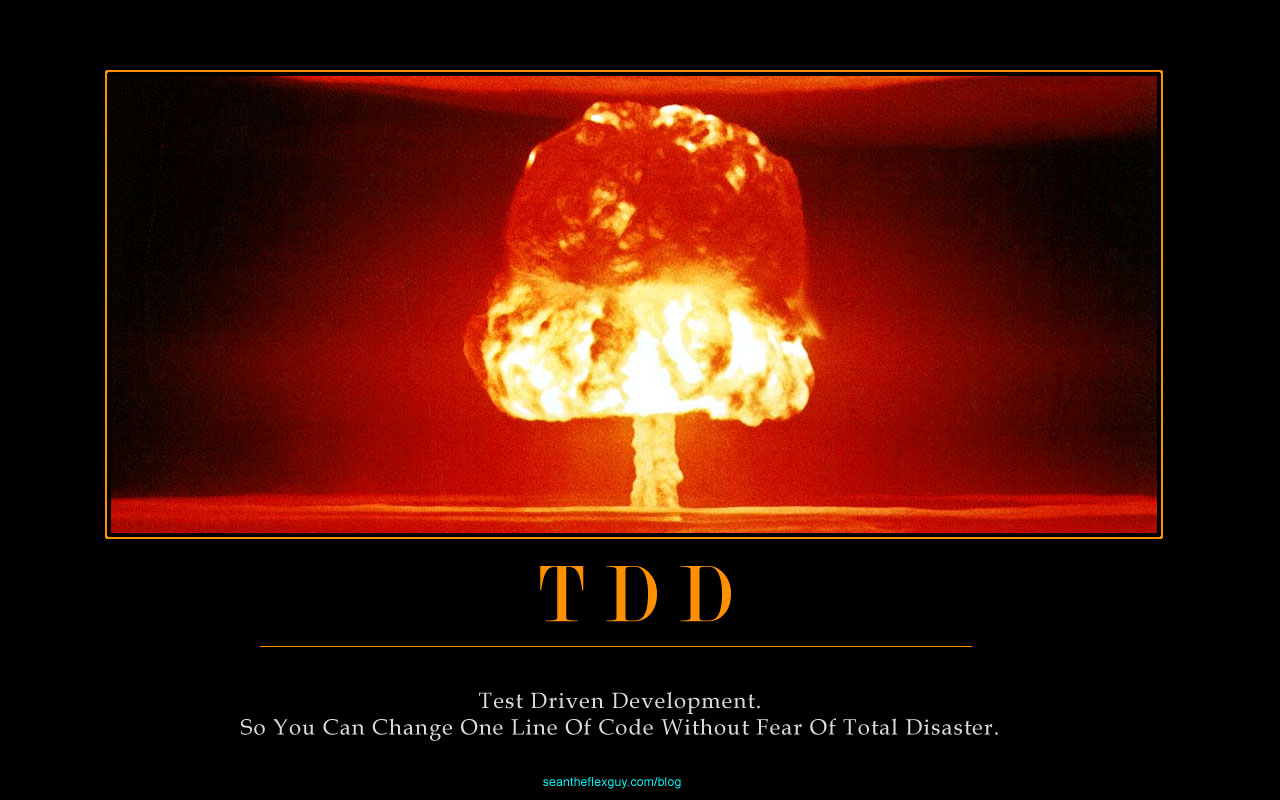
\includegraphics[width=\paperwidth, width=\paperwidth]{tdd.jpg}
\end{frame}





\end{document}
